In order to evaluate the training-modified versions of our extrapolation framework, we have to make sure that the evaluation data conforms to the restrictions that we apply to our training set to ensure consistency. In our first trainingmode, the used $N_\mathrm{max}$ are restricted to be lower than 24. In the second training mode, only interactions which are SRG evolved using a flow parameter of at least \srg{0.04} are used. Our evaluation set, consisting of $N_\mathrm{max}$ values up to 12 and of interactions evolved using a flow parameter of \srg{0.04} and \srg{0.08}, already satisfies these requirement.
\begin{figure}[H]
  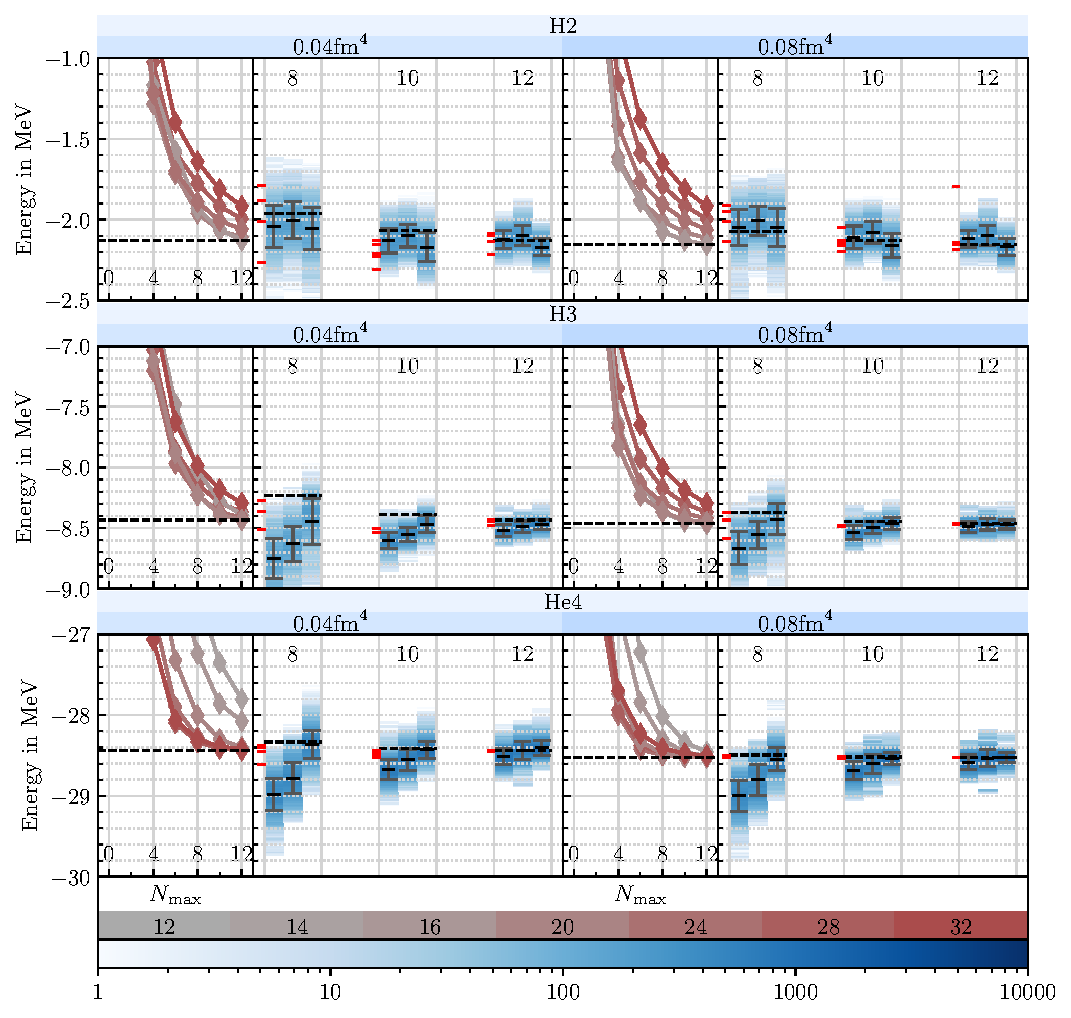
\includegraphics[width=\textwidth]{media/extended_evaluation.pdf}
  \caption{Evaluation of our training modes on the nuclei \n{2}{H}, \n{3}{H} and \n{4}{He}, using a semi-local momentum space regulated $N^2LO$ interaction with two-body interactions and a cutoff at \SI{450}{\mega\electronvolt}. The shown training modes are, in order from left to right, the basic training mode for comparison, the $N_\mathrm{max}$-limitation training mode and the SRG-filter training mode. For each nucleus and each flow parameter, the NCSM sequences are shown on the left (the different frequencies are colored respectively to the legend, which shows the frequencies $\hbar\Omega$ in \si[]{\mega\electronvolt}) and the extrapolations for a given maximum $N_\mathrm{max}$ on the right. For each maximum $N_\mathrm{max}$, the variational boundary is shown as a dashed line, and the classical extrapolations are shown as red ticks.}
  \label{fig:eval_extended}
\end{figure}

\autoref{fig:eval_extended} displays the evaluation of the three nuclei. Each histogram at every $N_\mathrm{max}$ is now divided into three seperate histograms, showcasing the evaluation result for the different training modes. In each stack of histograms, the leftmost is the basic training mode already introduced in \autoref{chap:framework} and assessed in \autoref{chap:reproduction}. The histogram in the center corresponds to our first training mode, which restricts the $N_\mathrm{max}$ in the training process to at most 24. The rightmost histogram is our second introduced training mode, which restricts the type of training interactions to SRG evolved interactions with a flow parameter of at least \srg{0.04}.

We again begin by looking at the nuclei \n{3}{H} and \n{4}{He}. For both training modes, we see that the predictions get closer to the variational boundary, which means that the training modes yield overall better predictions, since the sequences are already converged enough. Interestingly, the two trainingmodes seem to only impact the accuracy of the prediction. The uncertainty of both trainingmodes are comparable to the uncertainty of the prediction by the basic extrapolation framework.

If we compare the two trainingmodes for those nuclei, we see that the $N_\mathrm{max}$-limitation mode is less impactful than the SRG-filter mode. This can be explained by the fact that the some of the sequences of the \n{3}{H} and the \n{4}{He} nucleus are already converged enough. Since we explicitly remove bare Hamiltonians in the SRG-filter mode, the training set gets limited to a smaller size of fast converging sequences, thus training the net better to those cases. This can especially be seen in the \n{4}{He} nucleus, where there are sequences which have a very strong convergence rate. Here, the SRG-filter mode results lie very close to the variational boundary. The limitation on the $N_\mathrm{max}$ values also have a positive impact on the evaluation. This may indicate that the networks have learned from the constant sequences of high $N_\mathrm{max}$ values to linearly extrapolate the results up to a certain point, which results in the predictions being unreasonably low for low $N_\mathrm{max}$ sequences, as is the case for our basic extrapolation framework.
% 3h, 4he:
% nmax: a bit better
% srg: way better

For the nucleus \n{2}{H}, our basic framework showed a totally different systematic behaviour than for the nuclei \n{3}{H} and \n{4}{He}. This is also the case for both new training modes. Especially the $N_\mathrm{max}$ training mode seems to extrapolate not far enough, such that the predictions do not conform to the variational boundary at $N_\mathrm{max} = 12$. Even though the $N_\mathrm{max}$-limitation mode is thought to handle unconverged sequences better than the unmodified training mode, it predicts higher ground-state energies for both SRG flow parameters and for all $N_\mathrm{max}$ values. This can be explained by the fact that the \n{2}{H} sequences are not only converged until $N_\mathrm{max} = 12$, but also converge quite slowly. This leads to a very broad range of energy values at $N_\mathrm{max} = 12$ for all the frequencies, but the sequences themself are relatively flat, leading to a higher prediction of the $N_\mathrm{max}$-limitation training mode. The SRG-filter training mode seems to perform better than the basic training mode. Even though this training mode still produces unreasonably high predictions for $N_\mathrm{max} = 8$, the predictions for all $N_\mathrm{max} \geq 10$ are lower than the variational boundary at $N_\mathrm{max} = 12$. This is a great improvement over the other two training modes.

The comparison between the two different SRG flow parameters yield the same results as in the previous chapter, where we have considered our training without further modifications. We can see that the network predictions do not change much when evaluating the higher srg flow parameter. This is especially interesting in the case of \n{4}{He}, where the difference between the NCSM sequences is the biggest. At $\alpha = \srg{0.04}$, the lower sequences of $\hbar \Omega = \SI{12}{\mega\electronvolt}$ and \SI{14}{\mega\electronvolt} are converging fast, but they have not reached a sufficient degree of convergence, such that the values at $N_\mathrm{max} = 12$ are still spread far apart. For $\alpha = \srg{0.08}$, those sequences have converged sufficiently until $N_\mathrm{max} = 12$. We can see that the networks react very consistently between the different sequences.
% 2h:
% nmax worse than vanilla (WHY?)
% nmax geq 10: srg under varbound!

% difference srg
% same as vanilla: extrapolations go up


